\documentclass[11pt]{article}
\usepackage[utf8]{inputenc}
\usepackage[T1]{fontenc}
\usepackage{times}          % Fonte Times Roman (similar ao newtxtext)
\usepackage{mathptmx}       % Fonte matemática compatível
\usepackage{helvet}         % Opcional: Arial/Helvetica para sans-serif
\usepackage{amsmath}
\usepackage{multicol}
\usepackage{geometry}
\usepackage{tikz}
\usetikzlibrary{shapes.geometric, arrows.meta, 3d}
\usepackage{enumitem}
\usepackage{xcolor}
\usepackage{titlesec}

% Configurações de layout
\geometry{a4paper, left=1cm, right=1cm, top=0.5cm, bottom=1.2cm}
\setlength{\columnseprule}{0.4pt}
\setlength{\baselineskip}{1.0\baselineskip}

% Cores para títulos
\definecolor{myblue}{RGB}{0,0,128}
\definecolor{myred}{RGB}{200,0,0}
\titleformat{\section}{\normalfont\Large\bfseries\color{myblue}}{\thesection}{1em}{}
\titleformat{\subsection}{\normalfont\large\bfseries\color{myred}}{\thesubsection}{1em}{}
\titleformat{\subsubsection}{\normalfont\normalsize\bfseries\color{black}}{\thesubsubsection}{1em}{}

\title{\textcolor{myblue}{Geometria Espacial: Pirâmides}}
\author{Professor: Jefferson}
\date{}

\begin{document}

\maketitle
\vspace{-1cm}

\begin{center}
\large{Nome: \underline{\hspace{8cm}} \quad Turma: \underline{\hspace{3cm}} \quad Data: \underline{\hspace{3cm}}}
\end{center}

\begin{multicols}{2}

\section*{Introdução}
Uma \textbf{pirâmide} é um sólido geométrico formado por:
\begin{itemize}[leftmargin=*]
    \item Uma \textbf{base} poligonal (triangular, quadrangular, etc.)
    \item \textbf{Faces laterais} triangulares
    \item Um \textbf{vértice} comum chamado \textbf{ápice}
\end{itemize}

\begin{center}
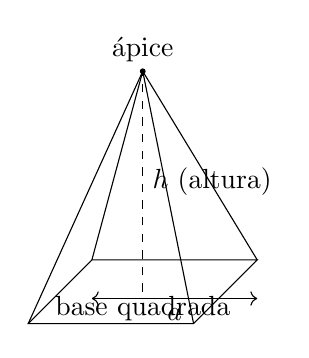
\begin{tikzpicture}[scale=0.7]
    % Base quadrada em perspectiva 3D
    \draw (0,0,0) -- (3,0,0) -- (3,0,3) -- (0,0,3) -- cycle;
    % Arestas laterais
    \draw (0,0,0) -- (1.5,4,1.5);
    \draw (3,0,0) -- (1.5,4,1.5);
    \draw (3,0,3) -- (1.5,4,1.5);
    \draw (0,0,3) -- (1.5,4,1.5);
    % Elementos
    \draw[dashed] (1.5,0,1.5) -- (1.5,4,1.5) node[midway,right] {$h$ (altura)};
    \filldraw (1.5,4,1.5) circle (1.2pt) node[above] {ápice};
    \node at (1.5,-0.3,1.5) {base quadrada};
    % Dimensões
    \draw[<->] (0,-0.7,0) -- (3,-0.7,0) node[midway,below] {$a$};
\end{tikzpicture}
\end{center}

\section*{Elementos Principais}
\begin{itemize}[leftmargin=*]
    \item \textbf{Altura} ($h$): distância do ápice ao plano da base
    \item \textbf{Apotema da base} ($a_b$): raio do círculo inscrito na base
    \item \textbf{Apotema da pirâmide} ($a_p$): altura das faces laterais
    \item \textbf{Aresta da base}: lado do polígono da base
    \item \textbf{Aresta lateral}: segmento do ápice a um vértice da base
\end{itemize}

\section*{Classificação}
\begin{itemize}[leftmargin=*]
    \item \textbf{Quanto à base}:
    \begin{itemize}
        \item Triangular (tetraedro)
        \item Quadrangular
        \item Pentagonal, etc.
    \end{itemize}
    \item \textbf{Quanto à inclinação}:
    \begin{itemize}
        \item Reta: pé da altura coincide com o centro da base
        \item Oblíqua: pé da altura não coincide com o centro
    \end{itemize}
\end{itemize}

\section*{Fórmulas Essenciais}
\subsection*{Áreas}
\[
\begin{aligned}
A_b &= \text{Área da base (depende do polígono)} \\
A_l &= \frac{P \times a_p}{2} \quad \text{(Área lateral)} \\
A_t &= A_b + A_l \quad \text{(Área total)}
\end{aligned}
\]

\subsection*{Volume}
\[
V = \frac{1}{3} \times A_b \times h
\]

\begin{center}
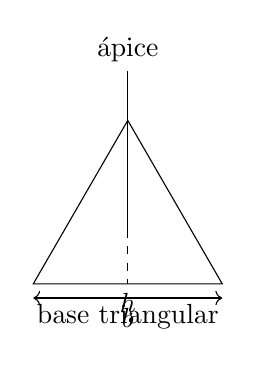
\begin{tikzpicture}[scale=0.6]
    % Pirâmide triangular
    \draw (0,0) -- (4,0) -- (2,3.46) -- cycle;
    \draw (2,1.15) -- (2,4.5) node[above] {ápice};
    \draw[dashed] (2,1.15) -- (2,0) node[below] {$h$};
    \node at (2,-0.7) {base triangular};
    \draw[<->] (0,-0.3) -- (4,-0.3) node[midway,below] {$b$};
\end{tikzpicture}
\end{center}

\section*{Relações Importantes}
Para pirâmides regulares:
\[
a_p^2 = h^2 + a_b^2 \quad \text{(Teorema de Pitágoras)}
\]

\section*{Atividades}
Calcule o que se pede em cada questão:

\begin{enumerate}[leftmargin=*]
    \item Uma pirâmide quadrangular regular tem aresta da base 5 cm e altura 12 cm. Qual seu volume?
    
    \item Determine a área total de uma pirâmide triangular regular com aresta da base 6 cm e apótema da pirâmide 5 cm.
    
    \item Uma pirâmide tem base retangular 4 cm × 9 cm e volume 60 cm³. Qual sua altura?
    
    \item Calcule o volume de uma pirâmide hexagonal regular com aresta da base 4 cm e altura $2\sqrt{5}$ cm.
    
    \item Qual a área lateral de uma pirâmide quadrangular regular com aresta da base 8 cm e apótema da pirâmide 10 cm?
    
    \item Uma pirâmide tem base quadrada de área 64 cm² e área total 144 cm². Qual a área lateral?
    
    \item Determine o volume de uma pirâmide com base triangular equilátera de lado 8 cm e altura 9 cm.
    
    \item Uma pirâmide regular tem volume 100 cm³ e altura 5 cm. Se a base é um pentágono regular, qual a área da base?
    
    \item Duas pirâmides têm mesma altura. Se as áreas de suas bases são 16 cm² e 25 cm², qual a razão entre seus volumes?
    
    \item Uma pirâmide quadrangular regular tem faces laterais que são triângulos equiláteros de lado 12 cm. Calcule seu volume.
\end{enumerate}

\section*{Gabarito}
\begin{enumerate}
    \item 100 cm³ \quad 2. $9\sqrt{3} + 45$ cm² \quad 3. 5 cm \quad 4. $48\sqrt{5}$ cm³ \quad 5. 160 cm²
    
    \item 80 cm² \quad 7. $48\sqrt{3}$ cm³ \quad 8. 60 cm² \quad 9. 16:25 \quad 10. $288\sqrt{2}$ cm³
\end{enumerate}

\section*{Resoluções Exemplares}
\subsection*{Questão 4}
\textbf{Dados:}
\begin{itemize}[leftmargin=*]
    \item Hexágono regular com $l = 4$ cm
    \item Altura $h = 2\sqrt{5}$ cm
\end{itemize}

\textbf{Passo 1:} Calcular área da base
\[
A_b = \frac{3\sqrt{3}}{2} \times l^2 = \frac{3\sqrt{3}}{2} \times 16 = 24\sqrt{3}\text{ cm}^2
\]

\textbf{Passo 2:} Calcular volume
\[
V = \frac{1}{3} \times 24\sqrt{3} \times 2\sqrt{5} = \frac{48\sqrt{15}}{3} = 16\sqrt{15}\text{ cm}^3
\]

\subsection*{Questão 10}
\textbf{Dados:}
\begin{itemize}[leftmargin=*]
    \item Faces laterais equiláteras com $l = 12$ cm
    \item Aresta da base = 12 cm
\end{itemize}

\textbf{Passo 1:} Calcular apótema ($a_p$)
\[
a_p = \frac{12\sqrt{3}}{2} = 6\sqrt{3}\text{ cm}
\]

\textbf{Passo 2:} Calcular altura ($h$)
\[
h = \sqrt{(6\sqrt{3})^2 - 6^2} = \sqrt{108 - 36} = 6\sqrt{2}\text{ cm}
\]

\textbf{Passo 3:} Calcular volume
\[
V = \frac{1}{3} \times 12^2 \times 6\sqrt{2} = \frac{144 \times 6\sqrt{2}}{3} = 288\sqrt{2}\text{ cm}^3
\]

\end{multicols}

\end{document}
